\documentclass[12pt]{article}
\usepackage{cmap}
\usepackage[T2A,T1]{fontenc}
\usepackage[english, russian]{babel}
\usepackage[utf8]{inputenc}

\usepackage{amsmath}
\usepackage{mathtools}

\usepackage{geometry}
\geometry{a4paper, left=1.2in, right=1in}

\usepackage{titlesec}
\titleformat{\section}
  {\normalfont\fontsize{21}{18}\bfseries}{\thesection}{1em}{}
  
\usepackage[bookmarks=false]{hyperref}
\hypersetup{pdfstartview={FitH},
            hidelinks,
            pdftitle={Отчет по индивидуальному заданию},
            pdfauthor={Павел Соболев}}
        
\usepackage{graphicx}
\usepackage[export]{adjustbox}
\graphicspath{{Plots/}}
            
\setlength\parindent{0pt}

\newcommand{\hl}[1]{(\hyperlink{eq:#1}{#1})}

\newcommand{\s}[2]{\hypertarget{skip:#1}{\vspace{#2pt}}}
\newcommand{\sd}[1]{\hypertarget{skip:#1}{\vspace{-10pt}}}

\newcommand{\hep}[2]{\vspace{#2pt}\hypertarget{eq:#1}{}\vspace{-#2pt}}

\newcommand{\hs}[1]{\sd{#1}\hep{#1}{18}}
\newcommand{\hst}[1]{\sd{#1}\hep{#1}{22}}
\newcommand{\he}[1]{\hep{#1}{18}}

\pdfsuppresswarningpagegroup=1

\begin{document}

\pagenumbering{Alph}
\thispdfpagelabel{Title}
\begin{titlepage}

    \newcommand{\HRule}{\rule{\linewidth}{0.5mm}}
    
    \center

    \ \\[6.5cm]
    
    \textsc{\Large Практикум анализа временных рядов}\\[0.5cm]
    
    \HRule\\[0.4cm]
    
    {\huge\bfseries Отчет по индивидуальному заданию}\\[0.4cm]
    
    \HRule\\[0.5cm]
    
    \large
    \textit{Автор:} Павел \textsc{Соболев}
    
    \ \\[0.9cm]
    \vfill\vfill\vfill
    
    {\large\today}
    
    \vfill
    
\end{titlepage}
\pagenumbering{arabic}

\subsection*{Часть 1}
\section*{Постановка и решение задачи}
\setcounter{section}{1}

\vspace{18pt}

Описание задачи из «В. В. Витязев — Спектрально-корреляционный анализ равномерных временных рядов», с. 41: \par

\vspace{\baselineskip}

Дан временной ряд $ x_k = x\left(\Delta t k\right), k = 0, 1, \ldots, 2N - 1 $, у которого первое и второе, третье и четвертое и т. д. значения попарно совпадают. Докажите аналитически, что периодограмма такого ряда будет симметрична относительно частоты $ \nu = 0.5 \nu_c = 1/4 \Delta t $. Проиллюстрируйте это свойство с помощью программы СКАВРя.

\subsection{Представление входных данных}

Имеем следующий временной ряд:

\hst{1}
\begin{gather}
    x_k = x\left(\Delta t k\right) , \hspace{8pt} k = 0, 1, \ldots, 2N - 1,
\end{gather}

для которого выполняется следующее свойство:

\hst{2}
\begin{gather}
    x_{2k} = x_{2k+1} \hspace{2pt} , \hspace{8pt} k = 0, 1, \ldots, N - 1.
\end{gather}

Объединяя с \hl{1}, получаем систему:

\hs{3}
\begin{gather}
    \begin{cases}
        x_k = x\left(\Delta t k\right) , \hspace{8pt} k = 0, 1, \ldots, 2N - 1; \\
        x_{2k} = x_{2k+1} \hspace{2pt} , \hspace{8pt} k = 0, 1, \ldots, N - 1,
    \end{cases}
\end{gather}

\vspace{5pt}

полностью описывающую входные данные, соответствующие условию задачи.

\subsection{Выполнение преобразования Фурье}

Имеем следующую формулу для вычисления периодограммы Шустера:

\hs{4}
\begin{gather}
    D(\nu) = \frac{1}{4 N^2} \left| \sum_{k = 0}^{2 N - 1} x_k e^{-i 2 \pi \nu \Delta t k} \right|^2.
\end{gather}

Введем обозначения:

\sd{5}
\begin{gather}
    X( \nu ) \coloneqq \sum_{k = 0}^{2 N - 1} x_k e^{-i 2 \pi \nu \Delta t k };
\end{gather}

\begin{minipage}[t][5pt]{10pt}
     
\end{minipage}

\vspace{-37pt}\hep{6}{20}
\begin{gather}
    X_{Re}(\nu) \coloneqq {Re}(X(\nu)) = \sum_{k = 0}^{2 N - 1} x_k \cos(2 \pi \nu \Delta t k);
\end{gather}

\s{7}{-20}
\begin{gather}
    X_{Im}(\nu) \coloneqq {Im}(X(\nu)) = - \sum_{k = 0}^{2 N - 1} x_k \sin(2 \pi \nu \Delta t k).
\end{gather}

Тогда выражение \hl{4} можно будет переписать как

\hs{8}
\begin{gather}
    D(\nu) = \frac{1}{4 N^2} | X(\nu) |^2 = \frac{1}{4 N^2} (X_{Re}^2(\nu) + X_{Im}^2(\nu)).
\end{gather}

\subsubsection{Вычисление $ X_{Re}^2(\nu) $}

Воспользуемся свойством \hl{2}, характерным исходному временному ряду \hl{3}, и преобразуем выражение \hl{6}:

\hst{9}
\begin{gather}
    X_{Re}(\nu) = \sum_{k = 0}^{N - 1} x_{2 k} [ \cos(2 \pi \nu \Delta t (2 k)) + \cos(2 \pi \nu \Delta t (2 k + 1) ].
\end{gather}

Воспользуемся тригонометрическим тождеством

\sd{10}
\begin{gather}
    \cos(\alpha) + \cos(\beta) = 2 \cos \frac{\alpha + \beta}{2} \cos \frac{\alpha - \beta}{2}
\end{gather}

и преобразуем \hl{9}:

\hst{11}
\begin{gather}
\begin{split}
    X_{Re}(\nu) &= 2 \sum_{k = 0}^{N - 1} x_{2 k} \cos\left( \frac{2 \pi \nu \Delta t (2k + 2k + 1)}{2} \right) \cos\left( \frac{2 \pi \nu \Delta t (2 k - 2 k - 1) }{2} \right) = \\
    &= 2 \sum_{k = 0}^{N - 1} x_{2 k} \cos( \pi \nu \Delta t (4k + 1) ) \cos( \pi \nu \Delta t) = \\
    &= 2 \cos( \pi \nu \Delta t) \sum_{k = 0}^{N - 1} x_{2 k} \cos( \pi \nu \Delta t (4k + 1) ).
\end{split}
\end{gather}

Возведем \hl{11} в квадрат:

\sd{12}\hep{12}{20}
\begin{gather}
    X_{Re}^2(\nu) = 4 \cos^2(\pi \nu \Delta t) \left[ \sum_{k = 0}^{N - 1} x_{2 k} \cos(\pi \nu \Delta t (4 k + 1) ) \right]^2.
\end{gather}

\subsubsection{Вычисление $ X_{Im}^2(\nu) $}

Аналогично предыдущему пункту получим выражение для $ X_{Im}(\nu) $, используя следующее тригонометрическое тождество:

\sd{13}
\begin{gather}
    \sin(\alpha) + \sin(\beta) = 2 \sin \frac{\alpha + \beta}{2} \cos \frac{\alpha - \beta}{2};
\end{gather}

\s{14}{-20}
\begin{gather}
    \begin{split}
    X_{Im}(\nu) &= - \sum_{k = 0}^{N - 1} x_{2 k} [ \sin(2 \pi \nu (2 k) \Delta t) + \sin(2 \pi \nu (2 k + 1) \Delta t) ] = \\
    &= - 2 \sum_{k = 0}^{N - 1} x_{2 k} \sin(\pi \nu \Delta t (4k + 1)) \cos(\pi \nu \Delta t) = \\
    &= - 2 \cos(\pi \nu \Delta t) \sum_{k = 0}^{N - 1} x_{2 k} \sin(\pi \nu \Delta t (4k + 1)).
    \end{split}
\end{gather}

Возводя результат в квадрат, получаем:

\hs{15}
\begin{gather}
    X_{Im}^2(\nu) = 4 \cos^2(\pi \nu \Delta t) \left[ \sum_{k = 0}^{N - 1} x_{2 k} \sin(\pi \nu \Delta t (4 k + 1) ) \right]^2.
\end{gather}

\subsubsection{Вычисление $ D(\nu) $}

Воспользуемся полученными выражениями \hl{12} и \hl{15} для вычисления \hl{8}:

\hs{16}
\begin{gather}
\begin{split}
    D(\nu) = \frac{\cos^2(\pi \nu \Delta t)}{N^2} & \left[ \left( \sum_{k = 0}^{N - 1} x_{2 k} \cos(\pi \nu \Delta t (4 k + 1)) \right)^2 + \right. \\
    & \hspace{7pt} \left. \left( \sum_{k = 0}^{N - 1} x_{2 k} \sin(\pi \nu \Delta t (4 k + 1)) \right)^2\right].
\end{split}
\end{gather}

\subsection{Поиск симметрии}

Рассмотрим подробнее суммы в выражении \hl{16}. Введем следующие обозначения:

\sd{17}
\begin{gather}
    S_{\cos}(\nu) \coloneqq \sum_{k = 0}^{N - 1} x_{2 k} \cos(\pi \nu \Delta t (4 k + 1));
\end{gather}

\sd{18}
\begin{gather}
    S_{\sin}(\nu) \coloneqq \sum_{k = 0}^{N - 1} x_{2 k} \sin(\pi \nu \Delta t (4 k + 1)).
\end{gather}

Проверим наличие симметрии относительно частоты $ 0.5 \nu_{c} $, где $ \nu_{c} $ -- частота Найквиста, равная $ 1 / (2 \Delta t) $:

\sd{19}\hep{19}{16.5}
\begin{gather}
    \begin{split}
    S_{\cos}(\nu_{c} - \nu) &= \sum_{k = 0}^{N - 1} x_{2 k} \cos(\pi (\nu_{c} - \nu) \Delta t (4 k + 1)) = \\
    &= \sum_{k = 0}^{N - 1} x_{2 k} \cos(\frac{\pi}{2} (4 k + 1) - \pi \nu \Delta t (4 k + 1))
    \end{split}
\end{gather}

\sd{20}\hep{20}{6}
\begin{gather}
    \begin{split}
    S_{\sin}(\nu_{c} - \nu) &= \sum_{k = 0}^{N - 1} x_{2 k} \sin(\pi (\nu_{c} - \nu) \Delta t (4 k + 1)) = \\
    &= \sum_{k = 0}^{N - 1} x_{2 k} \sin(\frac{\pi}{2} (4 k + 1) - \pi \nu \Delta t (4 k + 1))
    \end{split}
\end{gather}

Используя формулы приведения, упростим выражения \hl{19} и \hl{20}:

\sd{21}
\begin{gather}
    S_{\cos}(\nu_{c} - \nu) = \sum_{k = 0}^{N - 1} x_{2 k} \sin(\pi \nu \Delta t (4 k + 1));
\end{gather}

\sd{22}
\begin{gather}
    S_{\sin}(\nu_{c} - \nu) = \sum_{k = 0}^{N - 1} x_{2 k} \cos(\pi \nu \Delta t (4 k + 1)).
\end{gather}

Заметим следующее:

\sd{23}
\begin{gather}
    S_{\cos}(\nu) = S_{\sin}(\nu_{c} - \nu);
\end{gather}

\s{24}{-20}
\begin{gather}
    S_{\sin}(\nu) = S_{\cos}(\nu_{c} - \nu).
\end{gather}

Отсюда:

\hs{25}
\begin{gather}
    S_{\cos}^2(\nu) + S_{\sin}^2(\nu) = S_{\cos}^2(\nu_{c} - \nu) + S_{\sin}^2(\nu_{c} - \nu).
\end{gather}

Следовательно, значения, получаемые внутри квадратных скобок в выражении \hl{16}, симметричны относительно частоты, равной половине частоты Найквиста. \par

\vspace{\baselineskip}

Однако значения $ D(\nu) $ на частотах $ \nu $ и $ \nu_{c} - \nu $ не будут совпадать вследствие наличия множителя $ \cos^2(\pi \nu \Delta t) / N^2 $, также зависящего от частоты $ \nu $. Это значит, что пики, имеющиеся на частотах, меньших половины частоты Найквиста, будут отражены на симметричных относительно нее частотах с меньшей высотой. \par

\vspace{\baselineskip}

Множитель изменения высоты пика можно вычислить как

\hs{26}
\begin{gather}
    \Gamma = \frac{\cos^2(\pi (\nu_{c} - \nu) \Delta t) }{\cos^2(\pi \nu \Delta t) } = \frac{\sin^2(\pi \nu \Delta t) }{\cos^2(\pi \nu \Delta t) }.
\end{gather}

\newpage

\subsection*{Часть 2}
\section*{Практическое подтверждение}
\setcounter{section}{2}
\setcounter{subsection}{0}

\vspace{18pt}

Используемые далее графики получены с помощью программ с подключенным модулем SCATS, исходный код которого доступен в репозитории по адресу \\ \href{https://github.com/Paveloom/C3}{https://github.com/Paveloom/C3}. В частности, код для данной части отчета расположен в поддиректории «\href{https://github.com/Paveloom/C3/tree/master/%D0%A3%D0%BF%D1%80%D0%B0%D0%B6%D0%BD%D0%B5%D0%BD%D0%B8%D0%B5}{Упражнение}».

\subsection{Получение исходного ряда}

Как было видно в выкладках \hl{19} -- \hl{25}, свойство отражения значений функции $ S_{\cos}^2(\nu) + S_{\sin}^2(\nu) $ относительно частоты $ 0.5 \nu_{c} $ не зависит от функционального определения исходного временного ряда $ x_{k} $, а зависит только от того, удовлетворяет ли он системе \hl{3}. Тем не менее, желая иметь на периодограмме значимый пик, возьмем ряд, заданный следующим образом:

\hs{27}
\begin{gather}
    \begin{cases}
        x_k = A \cos(2 \pi \nu_{0} \Delta t k - \phi) , \hspace{8pt} k \% 2 = 0; \\
        x_k = A \cos(2 \pi \nu_{0} \Delta t (k - 1) - \phi) , \hspace{8pt} k \% 2 = 1; \\
        k = 0, 1, \ldots, 2 N - 1.
    \end{cases}
\end{gather}

Для такой системы выполняется свойство \hl{2}. Для определенности будем считать:

\hst{28}
\begin{gather}
    A = 1; \hspace{5pt} \nu_{0} = 0.125; \hspace{5pt} \Delta t = 1; \hspace{5pt} \phi = 0; \hspace{5pt} N = 256
\end{gather}

Сгенерированный таким образом ряд выглядит так:

\vspace{10pt}
\begin{minipage}[h]{\linewidth}
\center{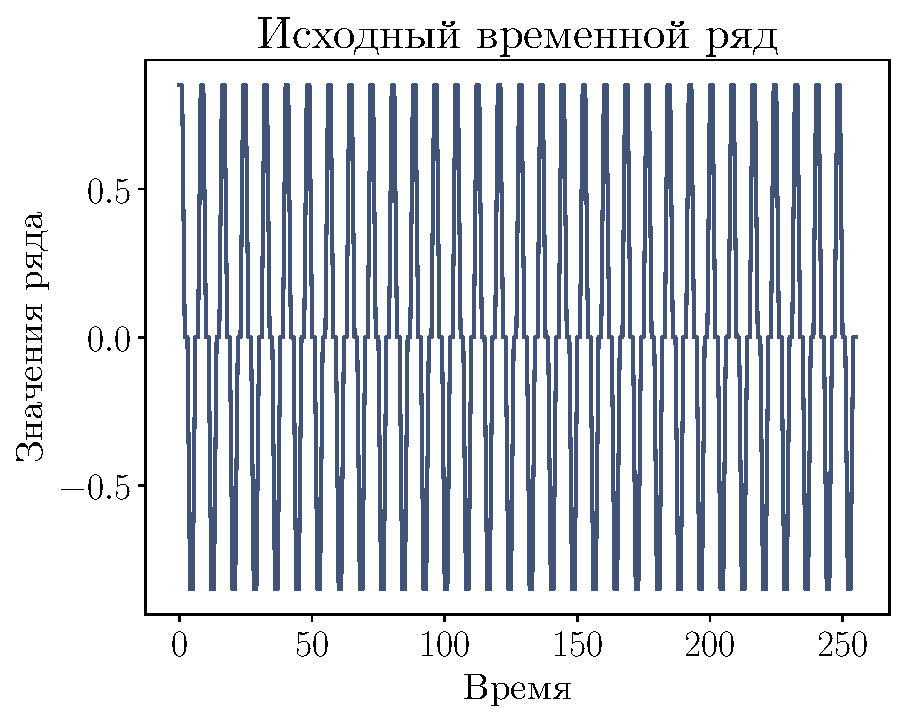
\includegraphics[totalheight=7.5cm]{input}}
\end{minipage}

\subsection{Вычисление периодограммы}

Покажем разницу между функциями $ S_{\cos}^2(\nu) + S_{\sin}^2(\nu) $ и $ D(\nu) $:

\vspace{10pt}
\begin{minipage}[h]{\linewidth}
\center{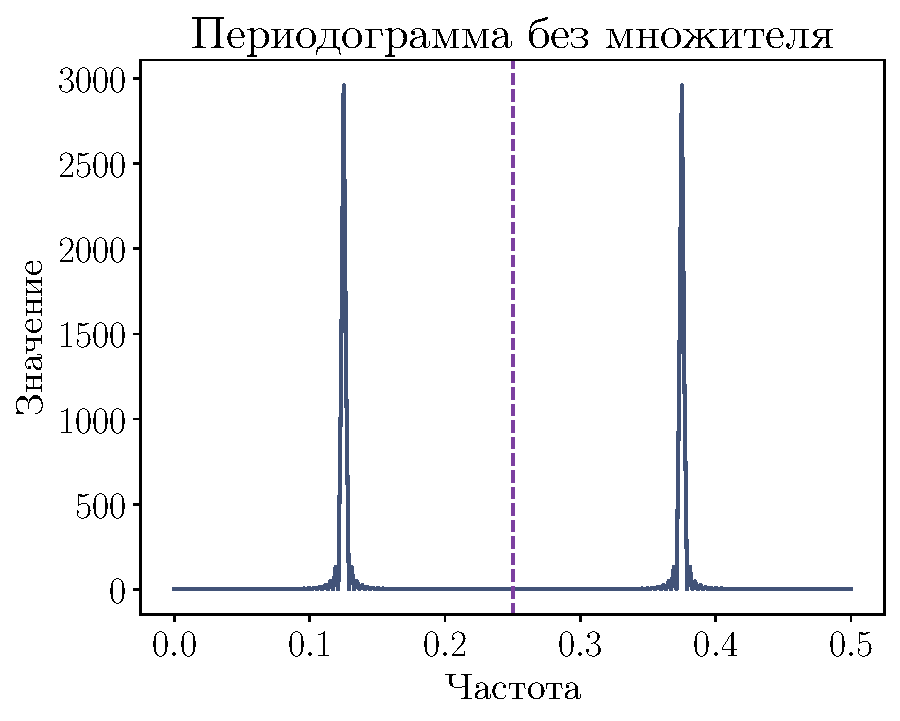
\includegraphics[totalheight=7.5cm]{S_2}}
\end{minipage}

\vspace{10pt}
\begin{minipage}[h]{\linewidth}
\center{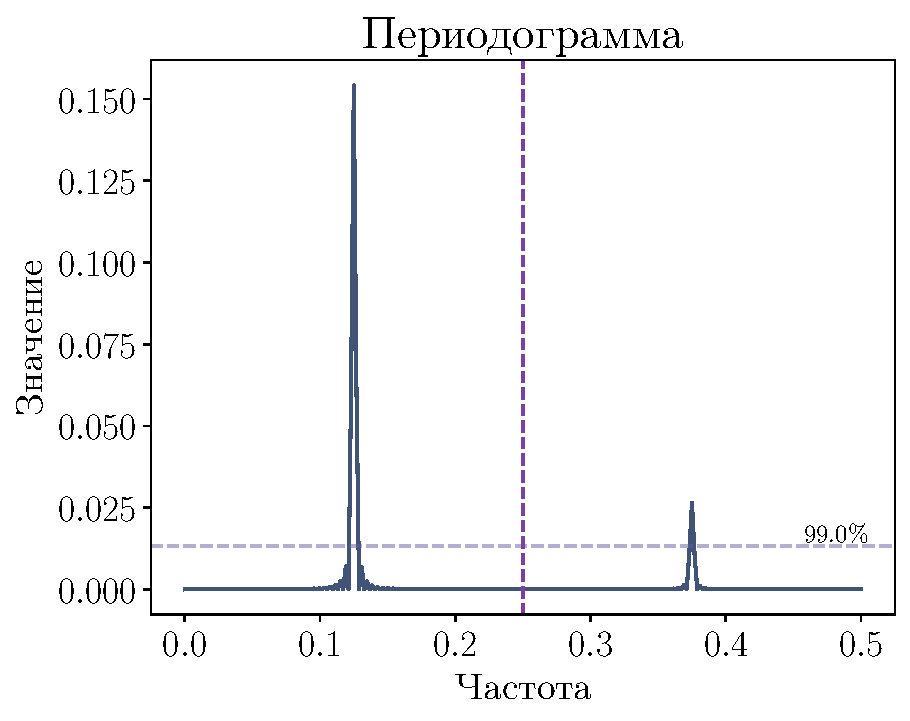
\includegraphics[totalheight=7.5cm]{periodogram}}
\end{minipage}

\vspace{\baselineskip}

Пунктирной вертикальной линией отмечена частота, равная половине частоты Найквиста. Получаем относительно нее симметрию значимого пика на графике функции $ S_{\cos}^2(\nu) + S_{\sin}^2(\nu) $, а на графике периодограммы отраженное значение обрезано множителем $ \cos^2(\pi \nu \Delta t) / N^2 $. Отношение $ \Gamma $ в данном случае равно $ \approx 0.1715729 $, что совпадает со значением выражения \hl{26} на частоте $ \nu_{0} $.

\subsection{Добавление шума}

Добавим шум во временной ряд \hl{27}, чтобы получить больше пиков на периодограмме:

\sd{29}
\begin{gather}
    \begin{cases}
        x_k = A \cos(2 \pi \nu_{0} \Delta t k - \phi) + \sigma_{x} \xi_{k} , \hspace{8pt} k \% 2 = 0; \\
        x_k = A \cos(2 \pi \nu_{0} \Delta t (k - 1) - \phi) + \sigma_{x} \xi_{k}, \hspace{8pt} k \% 2 = 1; \\
        k = 0, 1, \ldots, 2 N - 1,
    \end{cases}
\end{gather}

где $ \xi_{k} $ -- значения случайной величины, имеющей стандартное нормальное распределение, а

\sd{30}
\begin{gather}
    \sigma_{x} = \sqrt{\frac{A^2}{2 \gamma}} \mbox{ -- среднеквадратичное отклонение шумового компонента,}
\end{gather}

где $ \gamma $ -- отношение «сигнал к шуму». \par

\vspace{\baselineskip}

Возьмем ряд с теми же параметрами \hl{28}, а $ \gamma $ положим равным 0.5. \par

\vspace{\baselineskip}

С добавлением шума сгенерированный ранее ряд выглядит следующим образом:

\vspace{10pt}
\begin{minipage}[h]{\linewidth}
\center{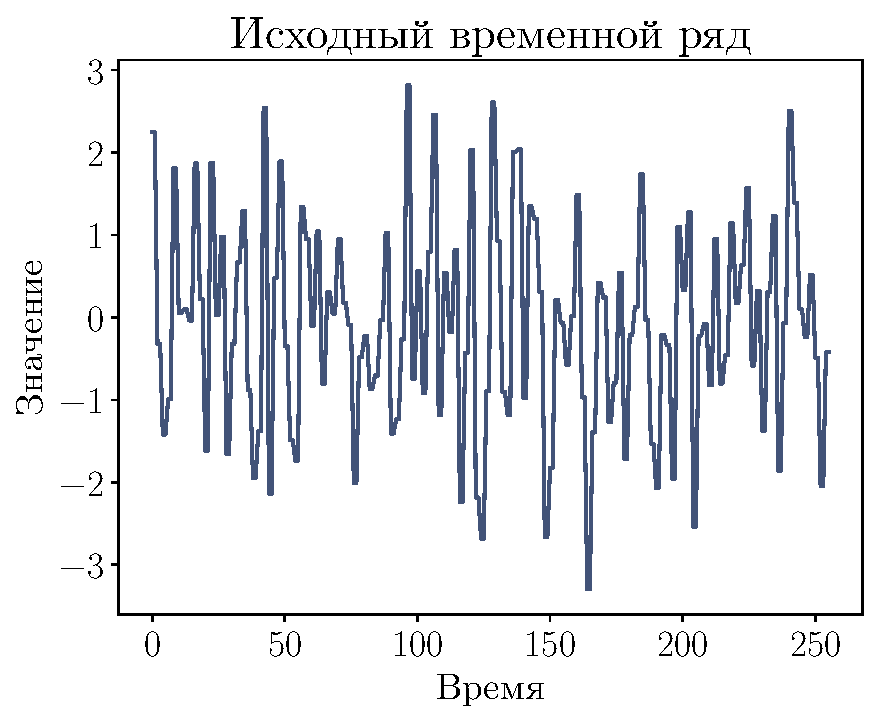
\includegraphics[totalheight=7.5cm]{input_noise}}
\end{minipage}

\subsection{Вычисление периодограммы с шумом}

Вновь сравним функции $ S_{\cos}^2(\nu) + S_{\sin}^2(\nu) $ и $ D(\nu) $:

\vspace{10pt}
\begin{minipage}[h]{\linewidth}
\center{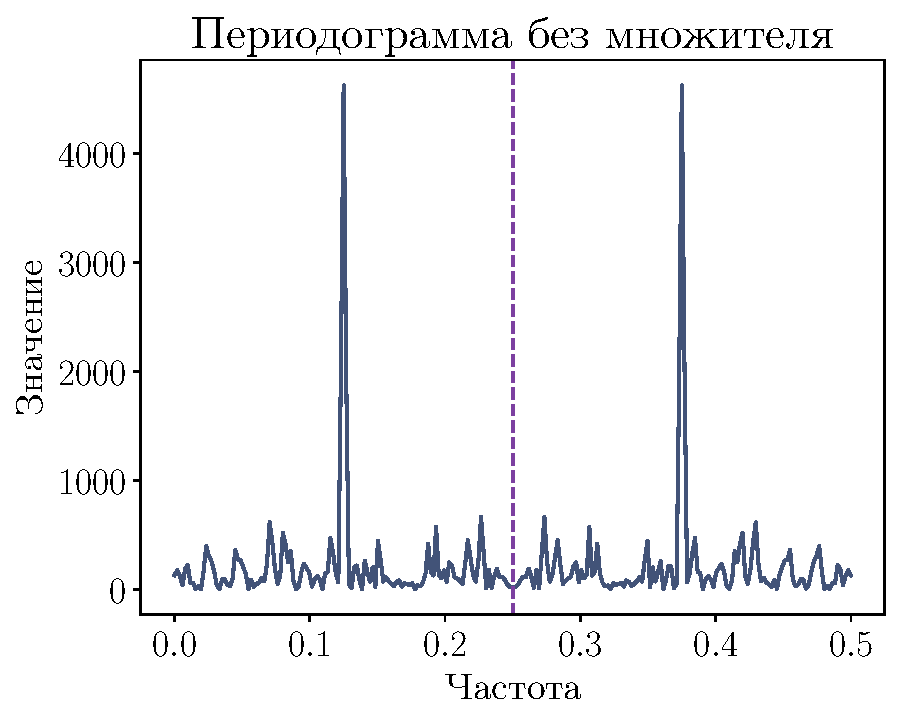
\includegraphics[totalheight=7.5cm]{S_2_noise}}
\end{minipage}

\vspace{10pt}
\begin{minipage}[h]{\linewidth}
\center{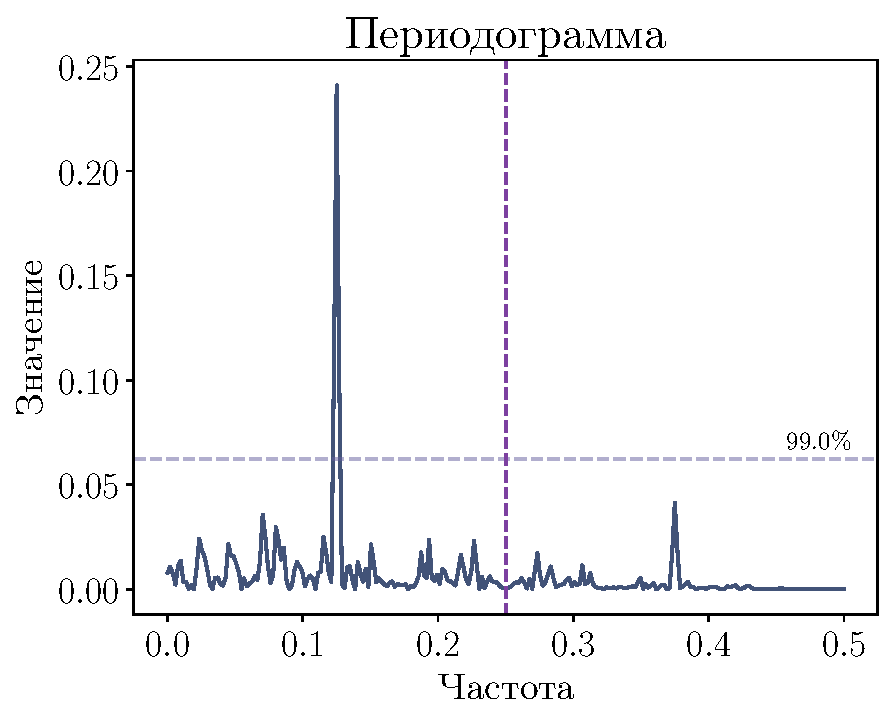
\includegraphics[totalheight=7.5cm]{periodogram_noise}}
\end{minipage}

\vspace{\baselineskip}

Видим, что каждый пик шума также имеет симметричное относительно половины частоты Найквиста отражение на графике функции $ S_{\cos}^2(\nu) + S_{\sin}^2(\nu) $. На графике периодограммы эти пики обрезаны множителем $ \cos^2(\pi \nu \Delta t) / N^2 $. \par

\vspace{\baselineskip}

Таким образом, практические результаты подтверждают теоретические.

\end{document}
